\documentclass{apuntes}

\title{Geometría Diferencial}
\author{Guillermo Julián Moreno}
\date{14/15 C2}

\usepackage{tikztools}
\usepackage{fastbuild}

% Paquetes adicionales

% --------------------

\begin{document}
\pagestyle{plain}
\maketitle

\tableofcontents
\newpage

\chapter{Formas diferenciales en abiertos de $ℝ^n$}

\section{Introducción y motivación}

Vamos a hacer un pequeño repaso de formas diferenciales. A lo largo de esta sección vamos a considerar la función $\appl{f}{U⊆ℝ^n}{ℝ}$, con $f∈C^∞(U)$.

Las formas diferenciales parten del concepto de derivadas y la búsqueda de ``tangentes'' a un punto. En esta línea, recordamos lo que es la matriz diferencial de una función que, por así decirlo, nos da la tasa de variación de una función cuando nos movemos a lo largo de un vector.

\begin{defn}[Diferencial\IS de una función] Dada $\appl{f}{U⊆ℝ^n}{ℝ}$, con $f∈C^∞(U)$ y $x_0 ∈ U$, entonces el diferencial en un punto es $\Dif f(x_0) = f'(x_0) = (\Dif f)_{x_0}$, que se considera como una aplicación lineal
\begin{align*}
\appl{\Dif f}{ℝ^n&}{ℝ} \\
(λ_1, \dotsc, λ_n)^T &\longmapsto \sum \dpa{f}{x_i} (x_0) λ_i
\end{align*}
\label{defDiferencialD}
\end{defn}

Hay que tener en cuenta que el espacio de partida de $\Dif f$, $ℝ^n$, no es el mismo espacio de partida de $f$. Diremos que el $ℝ^n$ de $\Dif f$ es el espacio tangente de $f$ en $x_0$ (denotado por $Π_{x_0} U = ℝ^n$).

Por ser una aplicación lineal de $ℝ^n$ en $ℝ$, el diferencial está en el espacio dual de $ℝ^n$ o, más concretamente, del espacio tangente de $U$: \[ \Dif f(x_0) ∈ \left(Π_{x_0} U\right)^* ≝ Π_{x_0}^* U\] donde $Π_{x_0}^* U$ será el espacio cotangente.

El espacio tangente se identifica con su dual no de forma única: depende de la elección de la base. Es decir, son isomorfos pero no son canónicamente isomorfos, ya que hay muchos isomorfismos y no hay uno privilegiado.

Para los que no recuerden cláramente qué es el espacio dual:

\begin{defn}[Espacio dual]
Dado cualquier espacio vectorial V sobre un cierto cuerpo F, definimos el \textbf{espacio dual V*} como el conjunto de todas las funcionales lineales en F, es decir, transformaciones lineales en V a valores escalares (en este contexto, un ``escalar'' es un miembro del cuerpo-base F). El propio V* se convierte en un espacio vectorial sobre F bajo la definiciones habituales ('punto a punto') de la adición y de la multiplicación escalar.
\end{defn}

Como el diferencial está en el espacio dual, sus elementos serán llamados \concept[Covector]{covectores}. Esto nos permitirá evitar líos de notación al considerar vectores en el espacio y por otro lado vectores en el espacio tangente.

Por otra parte, queremos introducir otra notación, la de las formas diferenciales, a partir de la diferencial exterior.

\begin{defn}[Diferencial\IS exterior] Dada $\appl{f}{U⊆ℝ^n}{ℝ}$, con $f∈C^∞(U)$ y $x_0 ∈ U$, entonces la diferencial en un punto es \[ (\dif f)_{x_0} = \sum \dpa{f}{x_i} (\dif x_i)_{x_0} \] En general, la diferencial será \[ \dif f = \sum \dpa{f}{x_i} \dif x_i \] \label{defDifrenciald}
\end{defn}

En realidad, la única diferencia entre esta definición y la dada en \ref{defDiferencialD} es que cambiamos los $λ_i$ por $\dif x_i$. En ambos casos tenemos, por definición, la diferencial es una 1-forma en el abierto $U$. Sabemos ya que una 1-forma es una expresión \[ ω = f_1 \dif x_1 + \dotsb + f_n \dif x_n \] con $f_i ∈ C^∞(U)$.

Cada $(\dif x_i)_{x_0}$ es un covector de $Π^*_{x_0}$, y de hecho $\set{(\dif x_i)_{x_0}}$ es una base del espacio de covectores.

\paragraph{Deducción de las reglas de cálculo} Vamos a considerar ahora una diferencial \[ \dif h = \dpa{h}{x_1} \dif x_1 + \dotsb + \dpa{h}{x_n} \dif x_n \] y una 1-forma \[ ω = f_1 \dif x_1 + \dotsb + f_n \dif x_n \]

Dado ω, nos preguntamos si existe una función $h$ tal que $\dif h = ω$. Es una propiedad muy deseable, porque nos da de alguna manera unas ciertas garantías de ``operación cerrada'' en formas diferenciales.

Esto es lo mismo que plantearse la resolución del sistema de ecuaciones diferenciales dado por \[ \dpa{h}{x_i} = f_i\quad i=1,2,\dotsc,n \]

Esta cuestión está resuelta por el teorema de Poincaré, que veremos más adelante durante el curso.

A primera vista, parece difícil que haya solución. Si uno elije las $f_i$ de forma aleatoria, tendremos demasiadas ecuaciones y pocas incógnitas. Luego debemos esperar condiciones de integrabilidad: las $f_i$ deben cumplir ciertas posibilidades para que la solución $h$ exista. Habitualmente estas condiciones son necesarias pero no siempre suficientes, y una vez que las encontremos suponemos que se cumplen (si no no hay solución) y veremos si bajo esas condiciones el problema tiene solución.

Dado que queremos que exista $h$, vamos a suponer que efectivamente existe $h$. Entonces va a ocurrir que $\dpa{h}{x_i} = f_i$, y si volvemos a derivar tendremos que $\frac{∂h}{∂x_j∂x_i} = \dpa{f_i}{x_j}$. Si derivamos en orden contrario, como el Teorema de Schwarz nos dice que las derivadas cruzadas son iguales, tendremos que tener \[ \dpa{f_i}{x_j} = \dpa{f_j}{x_i} \]

Hay una manera natural de poner toda esta información. Nosotros tenemos la matriz Hessiana de derivadas parciales segundas dada por \[ H = \left(\frac{∂h}{∂x_j∂x_i}\right)_{ij}\] que es simétrica por el Teorema de Schwarz.

Por otra parte, a partir de la forma diferencial $ω = f_1 \dif x_i + \dotsb + f_n \dif x_n$ podemos obtener la matriz $H_1$ dada por \[ H_1 = \del{\dpa{f_i}{x_j}}_{ij} \]

Habíamos visto que la diferencia entre la matriz diferencial y la diferencial exterior era simplemente de notación, luego parece lógico que $H = H_1$. Luego la condición de integrabilidad es que $H_1$ sea simétrica.

A partir de aquí podemos definir más formalmente la diferencial de una 1-forma

\begin{defn}[Diferencial\IS de una 1-forma] Dada una 1-forma ω, tenemos que \[ \dif ω ≝ H_1^Γ = \frac{H_1 - H^T_1}{2} \] donde $H_1^Γ$ es la parte antisimétrica de la matriz $H_1$.
\end{defn}

Esto nos lleva a poder dar una condición concreta para que exista la función $h$ que comentábamos antes. Como queremos que $H_1$ sea simétrica, la parte antisimétrica deberá ser 0. Podemos enunciar entonces el siguiente lema:

\begin{lemma} Si existe $h$ tal que $\dif h = ω$, entonces $\dif ω = 0$. \end{lemma}

Vamos a ver cómo aplicar todo ese tocho de antes para calcular la diferencial de una 1-forma $ω$ dada por \[ ω = f_1 \dif x_1 + f_2 \dif x_2 \] definida en un abierto $U ⊆ ℝ^2$. En este caso, su matriz $H_1$ será \[ H_1 = \begin{pmatrix} \dpa{f_1}{x_1} & \dpa{f_1}{x_2} \\ \dpa{f_2}{x_1} & \dpa{f_2}{x_2} \end{pmatrix} \] así que su parte antisimétrica será

\[ H_1^Γ = \begin{pmatrix} 0 & \displaystyle\frac{\dpa{f_1}{x_2} - \dpa{f_2}{x_1}}{2} \\ \displaystyle\frac{\dpa{f_2}{x_1}- \dpa{f_1}{x_2}}{2} \end{pmatrix} \]

Y como ese 2 molesta multiplicamos por dos y nos lo quitamos de en medio.

Como al diferenciar estamos derivando y la derivada es lineal, deberíamos esperar que \[ \dif ω = \dif (f_1\dif x_1) + \dif (f_2 \dif x_2)\] luego tenemos que ver cuánto vale $\dif(f_1\dif x_1)$.

Dado que la derivada tiene que seguir cumpliendo la regla de Leibniz, tenemos que tener \[ \dif(f_1\dif x_1) = \dif f_1 \dif x_1 + f_1 \dif \dif x_1 \]

Aquí ya empiezan a pasar cosas importantes de este cálculo de diferenciales. Principalmente que $ \dif \dif x_1 = 0$, ya que la matriz $H$ tiene que ser simétrica.

Ahora tenemos que calcular $ \dif f_1 \dif x_1 $, que será \[ \dif f_1 \dif x_1  = \left(\dpa{f_1}{x_1} \dif x_1 + \dpa{f_1}{x_2} \dif x_2\right)\dif x_1 = \dpa{f_1}{x_1}\dif x_1 \dif x_1 + \dpa{f_1}{x_2} \dif x_2 \dif x_1 \] luego sumando nos queda que

\[ \dif ω = \dpa{f_1}{x_1}\dif x_1 \dif x_1 + \dpa{f_1}{x_2} \dif x_2 \dif x_1  + \dpa{f_2}{x_1} \dif x_1 \dif x_2 + \dpa{f_2}{x_2} \dif x_2 \dif x_2 \]

Comparamos esto con la matriz antisimétrica dada por  \[ 2H_1^Γ = \begin{pmatrix} 0 & \dpa{f_1}{x_2} - \dpa{f_2}{x_1} \\ \dpa{f_2}{x_1}- \dpa{f_1}{x_2} & 0\end{pmatrix} \] vemos que los términos $\dpa{f_1}{x_1}$ y $\dpa{f_2}{x_2}$ no aparecen, luego tiene que ser \[ \dpa{f_1}{x_1} \dif x_1 \dif x_1 = \dpa{f_2}{x_2} \dif x_2 \dif x_2 = 0 \] y por otra parte que el producto de diferenciales tiene que ser anticonmutativo, esto es, que $\dif x_1 \dif x_2 = - \dif x_2 \dif x_1$. Dado que este producto (producto exterior) es distinto al habitual, lo denotaremos como $\dif x_1 \y \dif x_2$.

Es decir, hemos extraído las dos reglas siguientes para el producto de diferenciales o \concept[Producto\IS exterior]{producto exterior}: \begin{align*}
\df{x_i, x_j} &= - \df{x_j, x_i} \\
\df{x_i, x_i} &= 0
\end{align*}

Vamos a extendernos un poco en el significado de la expresión $\df{x_i, x_j}$, y por tanto en el de la forma diferencial. En el fondo, no estamos más que definiendo unos objetos (las formas) y aplicando ciertas reglas razonables para calcular ciertas operaciones. Ciertamente esto es cierto.

\paragraph{¿Es $\dif ω = 0$ condición suficiente?} Tenemos que es una condición necesaria para que exista un $h$ tal que $\dif h = ω$. Ahora bien, ¿es condición suficiente?

Para demostrarlo, lo que vamos a hacer es construir esa función $h$. Es trivial ver que \[ h(x) = \int_γ \dif h \] para un cierto camino $\appl{γ}{I}{U}$. En este caso, aplicando la regla de Barrow

\[ \int_γ \dif h = \int_I \dif(h ○ γ) = h(γ(b)) - h(γ(a)) = h(x) - h(x_0)\] donde $x_0$ es el punto de inicio de $γ$. Es decir, que $h$ está definido salvo constante. Habría que ver, eso sí, que la definición que hemos construído no depende de la elección del camino $γ$ y que, además, se cumple efectivamente que $\dif h = ω$.

Vamos a demostrar que la definición no depende del camino. Tomemos $γ_1, γ_2$ dos caminos distintos que empiezan y acaban en el mismo punto. Consideremos entonces $Γ = γ_1 * γ_2^-$, y sea $D$ la región encerrada por Γ.

Por un lado, tenemos que como $\dif ω = 0$, entonces $0 = \int_D \dif ω$. Por otra parte, por el teorema de Stokes, \[ \int_D \dif ω = \int_Γ ω = \int_{γ_1} ω - \int_{γ_2} ω \implies \int_{γ_1} ω = \int_{γ_2} ω\] luego la integral no depende del camino

Lo único que necesitamos para aplicar Stokes es que $U$ sea simplemente conexo, es decir, que no haya agujeros y que siempre podamos deformar un camino a otro, de tal forma que el borde de $D$ sea Γ.

En el fondo, esto es un reflejo de lo que habíamos visto en cursos anteriores de cálculo con campos de vectores conservativos: cuando eran conservativos ($\grad V = 0$) la integral sobre caminos cerrados era cero y además existía una función potencial.

\subsection{Resumen: reglas del cálculo de formas diferenciales}



\section{Estudio formal de las formas diferenciales}

\subsection{Espacio tangente y cotangente}

Suponemos un abierto $U ⊆ ℝ^n$ y un punto $p ∈ U$.

\begin{defn}[Espacio\IS tangente] Se define el espacio tangente de $U$ en un punto como $Π_{p} U$, un espacio vectorial sobre $ℝ$ de dimensión $n$. Los elementos $D^\vv_{p} ∈ Π_{p} U $ son las derivadas direccionales (en la dirección $\vv$) locales (en el punto $p$), que operan las funciones y dan números.
\end{defn}

Lo primero que nos damos cuenta es de que la derivada direccional es local, sólo definida en un entorno de $p$. Vamos por ello a tratar de definir este espacio tangente de forma algebraica, sin saltar al análisis. Y para ello empezaremos con conceptos de anillos de funciones, funciones definidas en intervalos.

\subsubsection{Anillo de funciones}

Si tenemos dos funciones $\appl{f,g}{U}{ℝ}$ definidas en el abierto $U$ con $f,g ∈ C^∞ (U)$, podemos operar con ellas de forma sencilla:

\begin{align*}
(f+g)(x) &≝ f(x) + g(x)
(f·g)(x) &≝ f(x) · g(x)
\end{align*}

Es decir, que las funciones definidas en el abierto tienen estructura de anillo: todas tienen inverso con la suma. Tenemos una unidad y además es anillo conmutativo. Así, podemos definir el anillo de funciones de un abierto:

\begin{defn}[Anillo\IS de funciones] El anillo de funciones de un abierto $U$ se define como

\[ A(U) = C^∞ (U) = \set{\appl{f}{U}{ℝ},\; f∈C^∞}\]

, que es anillo conmutativo y con unidad.\end{defn}

De hecho, $A(U)$ no es sólo un anillo: también es una \concept{{$\real$}-álgebra}: es un anillo conmutativo y además espacio vectorial sobre $ℝ$, cumpliendo la igualdad

\[ (λ· f) · (β·g) = (λ · β) · (f·g) \]

donde $f,g ∈ A(U)$, $λ,β ∈ ℝ$ y teniendo cuidado de usar los productos que correspondan\footnote{$(λ·_{E.V.} f) ·_{A(U)} (β·_{E.V.}g) = (λ ·_{\real} β) \cdot_{E.V.} (f·_{A(U)}g)$.} (el producto de elementos de $ℝ$ no es lo mismo que de elementos del anillo de funciones).

\subsubsection{Gérmenes de funciones en $p$}

La idea de los gérmenes es que sólo nos interesa la función en un entorno del punto. Podemos definir así entonces el germen como

\begin{defn}[Germen\IS de función] Un germen de una función en un punto $p$ es un par $(V,f)$ de un abierto $p ∈ V ⊆ U$ y una función $\appl{f}{V}{ℝ}$ con $f∈C^∞$. \label{defGermenFuncion}
\end{defn}

La razón de buscar esta definición es que para la derivada no necesitamos definir la función en todo $U$, nos basta con sólo un poco, y eso nos facilitará las cosas.

Ahora bien, los gérmenes de funciones en realidad se trabajan con relaciones de equivalencia para simplificar. Diremos que dos gérmenes $(V,f)$, $(W,g)$ están relacionados ($(V,f) \sim (W,g)$) si y sólo si $p∈V∩W$ y además existe un abierto $V' ⊆ V∩W$ que contiene a $p$ y para el cual las restricciones de $f$ y $g$ coinciden, esto es $\restr{f}{V'} = \restr{g}{V'}$.

Tomando los gérmenes módulo esta relación de equivalencia, tendremos igualmente una $\real$-álgebra.

La ventaja de buscar ese abierto más pequeño es que no tenemos que decir exactamente cómo de pequeño es, nos basta simplemente que las funciones sean iguales en un pequeño entorno del punto.

A partir de esto, denotaremos como $A_p$ la $\real$-álgebra de gérmenes de funciones $C^∞$ definidas en un entorno de $p$. Por comodidad, para denotar un germen nos bastará con la función, $f∈A_p$, por ejemplo. También podemos pasar a definir lo que es una derivación:

\begin{defn}[Derivación] Una derivación en $p$ es una aplicación
\begin{align*}
\appl{D}{A_p&}{ℝ} \\
f &\longmapsto D(f)
\end{align*}

Queremos que esta función conserve de alguna forma la noción de derivada en una dirección, así que buscaremos varias propiedades:

\begin{enumerate}
	\item $D$ es lineal.
	\item $D(λ) = 0$, donde $λ$ es una función constante $λ(x) = λ ∈ ℝ$.\footnote{En realidad, esta propiedad es consecuencia de las otras dos pero viene bien tenerla presente.}
	\item Si esto se parece una derivada, además de definir cómo se derivan las sumas\footnote{Por esto forzamos que $D$ sea lineal.} definiremos cómo se derivan los productos, según la regla de Leibniz: \[ D(f·g) = f · D(g) + D(f) · g\]
\end{enumerate}\label{defDerivacion}
\end{defn}

Una vez que hemos emulado las derivadas, podemos definir el espacio tangente:

\begin{defn}[Espacio\IS tangente] Diremos que el espacio tangente a $p$ en $U$ se define como

\[ Π_p U ≝ \set{\appl{D}{A_p}{ℝ}\tq D \text{ derivación }} \]
\end{defn}

Fijémonos que el espacio tangente es un subespacio vectorial del espacio dual, ya que $A^*_p ≝ \set{\appl{D}{A_p}{ℝ} \tq D \text{ lineal }}$. De hecho, tenemos bien definido el producto por escalares y la suma de elementos de la forma habitual.

\paragraph{Motivación de todo esto} Al final, hemos logrado llegar a una definición de espacio tangente sin tener que usar derivadas, una definición puramente algebraica.

Con esta definición algebraica vamos a estudiar el espacio tangente, principalmente su dimensión, y vamos a obtener una base cómoda para hacer cálculos.

\subsubsection{Cálculo de la dimensión del espacio tangente}
\label{secDimTangente}

Vamos a demostrar que la dimensión del espacio tangente de un abierto de $ℝ^n$ es $n$. Suponemos $p ∈ U ⊆ ℝ^n$, y $p = (p_1, \dotsc, p_n)$. Supongamos también que tenemos una derivación $\appl{D}{A_p}{ℝ}$. Vamos a ver qué podemos obtener de aquí sabiendo las propiedades de la derivación.

La observación fundamental es que en el conjunto de gérmenes $A_p$ tenemos un cierto subconjunto en los que el germen es 0: \[ m_p ≝ \set{f ∈ A_p \tq f(p) = 0}\] que además es un ideal por la propia construcción. Y resulta ser maximal\footnote{Aunque todos nos acordamos de Estructuras Algebraicas, recordamos por si acaso: un ideal es maximal si no hay ningún ideal propio que lo contenga.}, ya que el cociente $\quot{A_p}{m_p}$ es un cuerpo: por construcción, las clases de equivalencia estarán formadas por funciones cuya diferencia sea constante, luego $\quot{A_p}{m_p} = ℝ$, que es un cuerpo.

Aquí no sé qué está haciendo: $D(λ) = 0$. $m_p ⊃ m_p^2$, donde $m_p^2$ es el ideal generado por productos de elementos de $m_p$, esto es, \( \label{eqMp2} m_p^2 ≝ \set{\sum g_{ij} f_i f_j \tq f_i f_j ∈ m_p }\)

¿Qué ocurre si derivamos $f·g$ con $f,g ∈ m_p$? Por la regla de Leibniz, tenemos que \[ D(f·g) = d· D(g) + g · D(f) \] Como $f = g = 0$, tenemos que $D(f·g) = 0$. Entonces es claro que cuando aplicamos la derivación a elementos de $m_p^2$ nos sale 0. La conclusión de todo esto es que $\restr{D}{m_p^2} \equiv 0$. Es decir, que la regla de Leibniz nos nosequé algo sobre cosas finitas y espacios enormes. Que eso nos lleva a que $D$ está determinada en realidad por los valores que toma en $\quot{A_p}{m_p^2}$. Es decir, que si denotamos
\begin{align*}
\appl{D}{A_p&}{ℝ} \\
\appl{π}{A_p&}{\quot{A_p}{m_p^2}} \\
\appl{\adh{D}}{\quot{A_p}{m_p^2}&}{ℝ}
\end{align*} nos queda que \[ D(f) = \adh{D}(π(f)) \]

Al final, hay un motivo por el cual este chorro nos dice que algo es finito.

El argumento es que una derivación $\appl{D}{A_p}{ℝ}$ induce una aplicación $\appl{\adh{D}}{\quot{A_p}{m_p^2}}{ℝ}$, que se puede ver de otra forma como $\appl{\adh{D}}{\quot{m_p}{m_p^2}}{ℝ}$ ya que si $f ∈ A_p \setminus m_p$ $D(f) = 0$. Entonces $\adh{D}$ es, por construcción, un elemento del espacio vectorial de $\quot{m_p}{m_p^2}$, y además a partir de $\adh{D}$ podemos reconstruir la $D$ original.

Veamos cómo hacer eso mismo: si tenemos $f∈A_p$ con $f(p) ≠ 0$, entonces consideramos la función $f_1(x) ≝ f(x) - f(p)$. Entonces $f_1(x) ∈ m_p$ por construcción\footnote{Recordamos que $m_p$ son las funciones que se anulan en $p$.}. Es claro que yo debo definir \[ D(f) ≝ \adh{D}\left([f_1]_{m^2_p}\right) \]

Es decir, que sólo con saber lo que vale $\adh{D}$ nos vale ya que simplemente trasladamos las funciones $f$ con valores desconocidos $f ∉ m_p$ a una clase de equivalencia de la cual sí sabemos el valor. Sólo tenemos que ver que efectivamente cumple la propiedades de derivación que habíamos pedido (\ref{defDerivacion}). Es trivial ver que se cumple la linealidad, pero Leibniz es más interesante. Empezamos\footnote{Se ve que por comodidad estamos escribiendo $f(x) \equiv f$.} con

\[ D(f·g) = \adh{D}\left([f·g - f(p) g(p)]_{m_p^2}\right) \]

¿Qué hacemos ahora\footnote{Sugerencia de Guille: llorar y dedicarnos a magisterio.}? Sólo sabemos que $\adh{D}$ es lineal. Podemos fijarnos en que \[ α = (f-f(p))· (g-g(p)) ∈ m_p^2\] por ser producto de funciones de $m_p$, luego $\adh{D}(α) = 0$. Si operamos, nos queda \[ (fg - f(p) g - g(p) f + f(p) g(p) \] y si obtenemos su derivación tenemos que

\[ \adh{D}(α) = \adh{D}(f·g) - f(p) \adh{D}(g) - g(p)\adh{D}(f) + \adh{D}(f(p)· g(p)) \]

\begin{example}[Estudio del espacio tangente con funciones polinomiales]

Vamos a suponer que trabajamos con polinomios (espacio $ℝ[x,y]$), que son más sencillos: con ellos podemos derivar formalmente sin definiciones de límites ni nada, y además, los gérmenes son los mismos polinomios: si tenemos todos los valores que toma en un abierto de $ℝ$, tenemos completamente determinado el polinomio.

Supongamos $p = (0,0)$. Entonces, ¿qué es $m_p ⊆ ℝ[x,y]$? Será\footnote{Teniendo en cuenta que $p(x,y) = a_0 + a_1 x + a_2 y + \dotsb$} \[m_p = \set{p(x,y) ∈ ℝ[x,y] \tq p(0,0) = 0} = \set{p(x,y) \tq a_0 = 0} \]

Queremos ver qué es $m_p^2$. Está claro que $x^2, y^2, xy ∈ m_p^2$. Afirmamos que $m_p^2 = \gen{x^2, y^2, xy}$, y vamos a demostrarlo. Si fuese así y tuviésemos $F(x,y) ∈ m_p^2$, podríamos escribirlo como \[ F(x,y) = \sum A_{ij}(x,y) · p(x,y) · q(x,y) \] siguiendo la definición que teníamos en \eqref{eqMp2}, y con $p, q ∈ m_p$. Por lo tanto, $p,q$ sólo pueden ser polinomios con término independiente 0 y entonces nos quedaría que efectivamente

\[ m_p^2 = \gen{x^2 + y^2 + xy} = \set{A(x,y) x^2 + B(x,y) y^2 + C(x,y) xy} \]

Una vez que tenemos $m_p$, queremos ver quién es $\quot{m_p}{m_p^2}$, que es el espacio cotangente a algo $Π_{(0,0)}^*$. Si $p(x) ∈ m_p^2$, entonces \[ p(x) = a_1 x + a_2 y + a_3 x^2 + a_4 xy + \dotsb \] Si $p, q$ están en la misma clase de equivalencia, su resta tiene que estar en $m_p^2$, luego los polinomios $r(x) ∈ \quot{m_p}{m_p^2}$ son de la forma \[ r(x) = a_1 x + a_2 y\] o, dicho de otra forma, \[ \quot{m_p}{m_p^2} \equiv ℝ·[x] + ℝ· [y] \] Es decir, que estamos en un espacio de dimensión dos que es lo que tenía que ser.
\end{example}

Una vez que hemos logrado manejar algo mejor y ver la aplicación de todos estos conceptos, podemos pasar a la formalización de la demostración de la dimensión del espacio tangente.

\begin{theorem} \label{thmDimQuotMp} Sea $p ∈ U ⊆ ℝ^n$, con $p = (x_1, x_2, \dotsc, x_n)$. Entonces el espacio $\quot{m_p}{m_p^2}$ es un R-espacio vectorial de dimensión $n$.\end{theorem}

Hasta ahora todo lo que hemos visto han sido manipulaciones algebraicas, aunque para demostrar este teorema hace falta usar análisis.

\begin{proof}[Idea] Suponemos que $n = 1$, y consideramos el desarrollo de Taylor de una función $f ∈ A_p$:

\[ f(x) - f(p) = f'(p)(x - p) + \frac{1}{2!} f''(p)(x - p)^2 + \dotsb\]

Vemos que $f''(p)(x - p)^2  ∈ m_p^2$. Dado que trabajamos en módulo $m_p^2$, tenemos que $[f(x) - f(p)] = f'(p) [ x- p]$. Esto demuestra que $\quot{m_p}{m_p^2}$ tiene base $[x - p]$, luego efectivamente la dimesión es 1.

Vamos ahora con la demostración más rigurosa. Para una función $f ∈ A_p$, tenemos\footnote{ Por el teorema de Taylor e incluyendo el término de error, en este caso con la formulación integral } que

\[ f(x) - f(p) = \sum_{i=1}^n \dpa{f}{x_i} (x_i - p_i) + \sum_{\substack{i=1 \\ j=1}}^n \frac{1}{2} (x_i - p_i)(x_j - p_j) ·\int_0^1 (1-t) \left(\frac{∂^2f}{∂x_i ∂x_j}(p + tx)\right) \dif t \]

Entonces nos queda que \[ [f(x) - f(p)] = \sum_{i=1}^n \dpa{f}{x_i} (p) [x_i - p_i] \mod m_p^2 \] así que está claro que $\set{[x_i-p_i]}_{i=1}^n$ son generadores de $\quot{m_p}{m_p^2}$. No hemos demostrado que sean base, eso sí.

Para terminar, demostramos que ese conjunto de generadores son linealmente independientes y que por lo tanto serán base. Lo haremos por demostración al absurdo: si no fueran independientes, podríamos tener una función \[ F = \sum λ_i (x_i - p_i) ∈m_p^2\]

Esto es un poco absurdo ya de por sí\footnote{El profesor ha dicho por qué pero yo no lo veo nada claro.}, pero vamos a demostrarlo.

Sabemos que $∀D$ $D(F) = 0$. Entonces, elegimos un conjunto de derivaciones $D_j$ tales que $D_j ( x_i - p_i) = δ_{ij}$ con $δ$ la delta de Kronecker (ver \ref{defDeltaKronecker}). En ese caso, \[ D_j(F) = \sum λ_i D_j (x_i - p_i) = λ_j\] pero hemos dicho que $D(F) = 0$, contradicción.

¿Qué $D_j$ nos valen? Si tomamos $D_j = \left(\dpa{}{x_j}\right)_p$, cumplen las propiedades de derivación y también que $D_j (x_i - p_i) = \dpa{(x_i - p_i)}{x_j} = δ_{ij}$\footnote{Es fácil ver que $D_j(x_i - p_i)$ será 1 cuando $j = i$.}.

En ese caso, tenemos efectivamente que $\set{[x_i-p_i]}_{i=1}^n$ es base.
\end{proof}

Con esta demostración hemos llegado a algo interesante, que es ver qué es un diferencial de cada coordenada \[ (\dif x_i)_p ≝ [x_i - p_i]_{m_p^2} \] y, de la misma forma, el diferencial de una función \[ (\dif f)_p ≝ \left[f - f(p)\right]_{m_p^2} ∈ \quot{m_p}{m_p^2} \]

De esta notación y del teorema anterior \ref{thmDimQuotMp} podemos llegar a otra notación:

\( (\dif f)_p = \sum \dpa{f}{x_i}(p) (\dif x_i)_p \label{eqDiferencialNotacion} \)

En realidad, lo que estamos haciendo es similar a un desarrollo de Taylor despreciando los términos de segundo orden (que es lo que logramos con el módulo $m_p^2$): aproximaciones lineales de funciones.

De momento estamos trabajando localmente, siempre con la diferencial definida en un punto $p$. Pronto pasaremos a definir las diferenciales en abiertos o incluso en variedades directamente.

\subsubsection{Construcción del espacio tangente}

Recapitulemos: hemos demostrado hasta ahora el siguiente isomorfismo entre el espacio tangente y el dual  \[ Π_p U \simeq \left(\quot{m_p}{m_p^2}\right)^* \] que $\dim_{ℝ} \quot{m_p}{m_p^2} = n$ y que además hay una base natural \[ \quot{m_p}{m_p^2} = \gen{(\dif x_1)_p, \dotsc, (\dif x_n)_p} \]

A partir de aquí también podemos escribir una base del tangente $Π_p U$. Como podemos identificar el tangente con el dual de $\quot{m_p}{m_p^2}$, si definimos $\set{(D_i)_p}_{i=1}^n$ como la base de $Π_p U$, tenemos que cada $D_i$ tiene que ser un elemento del dual\footnote{Me estoy perdiendo mucho.}: \[ (D_i)_p (x_j - x_j(p)) = δ_{ij}\] aunque por notación más cómoda tomaremos \[ (D_i)_p ≝ \left(\dpa{}{x_i}\right)_p \] y por lo tanto podemos reescribir la base del espacio tangente en un punto como \[ Π_pU = \gen{\left(\dpa{}{x_1}\right)_p, \dotsc, \left(\dpa{}{x_n}\right)} \] y entendiendo cada $\left(\dpa{}{x_i}\right)_p$ como derivaciones lineales que se aplican a gérmenes de funcioens de $p$ y que cumplen la regla de Leibniz.

Así, cualquier elemento $D_p ∈ Π_p U$ se puede expresar como  \[ D_p = \sum a_i \left(\dpa{}{x_i}\right)_p \] con $a_i ∈ ℝ$.

De hecho, como cada $D_p$ sólo tiene la información de los $a_i$, podemos considerar los $D_p$ como vectores del espacio ambiente $ℝ^n$. Análogamente, se puede obtener cada coordenada del vector tangente derivando con respecto a las coordenadas en $U$: \[ D_p (x_j) = a_j \]

Podemos preguntarnos por qué tanto lío para llegar al final a que los elementos del espacio tangente son vectores de $ℝ^n$. La respuesta si nos da por hacer eso es que de esta forma tenemos una definición estricta y formal de las formas diferenciales que nos permitirá extenderlas naturalmente\footnote{Naturalmente mis narices.} a variedades.

Otra forma de definir esto sería usar clases de equivalencia de curvas, construyendo vectores tangentes sin acabar de hablar de tangentes. Veremos (y el profesor espera convencernos de eso) que esta forma que hemos desarrollado es en realidad mejor, ya que se comportan mejor respecto a ciertas operaciones. No es lo estándar, desde luego, pero de hecho se va imponiendo que es mejor.\footnote{Resumen: las formas molan y los tensores son caca.}

\subsection{Relación con cálculo}

Suponemos que tenemos abiertos $U⊆ℝ^n, V⊆ℝ^m$, y una aplicación $\appl{F}{U}{V}$ con $F ∈ C^∞$. Sea $p ∈U$ y $F(p) ∈V$, y supongamos $D_p$ un vector tangente (o derivación) en $p$. La pregunta es si le podemos asociar una derivación en $F(p)$, o dicho de otra forma, si $F$ manda vectores tangentes en vectores tangentes.

Esto puede ocurrir o no, pero como pregunta es importante. Lo que haremos será estudiar variedades y funciones entre variedades, y ver si las propiedades del cálculo diferencial se mantienen por funciones.

Definiremos entonces $F_{*,p}(D_p)$ como un vector tangente a $F(p)$ en $V$. Este elemento existe, se podrá definir con una fórmula, y se podrá aplicar a funciones $g ∈ A_{F(p)}$ donde $A_{F(p)}$ es el conjunto de gérmenes de funciones en $F_{(p)}$ (ver \ref{defGermenFuncion}).

Sabemos derivar en $U$ pero no en $V$, entonces lo que vamos a hacer va a ser una permutación de símbolos que tiene sentido\footnote{Metageometría diferencial.}. En este caso, nos queda \[ F_{*,p}(D_p)(g) = D_p (g ○ F)\] donde $g ○ F ∈ A_p$ y sí sabremos derivarlo. Queda demostrar que efectivamente $F_{*,p}(D_p)$ es una derivación\footnote{Se deja como ejercicio.}. Con la suma, tendríamos algo como esto:

\[ F_{*,p}(D_p + D_p')(g) = [D_p + D_p'](g○F) \]

Querríamos escribir ahora  $[D_p + D_p'](g○F) = D_p (g○F) + D_p'(g○F)$, y de hecho podemos hacerlo por ser $D_p, D_p'$ elementos del dual de los gérmenes y por la definición de la suma en el dual\footnotemark y por lo tanto nos quedaría efectivamente que \[ F_{*,p}(D_p + D_p')(g) = F_{*,p}(D_p)(g) + F_{*,p}(D_p')(g) \]

\footnotetext{La suma de dos elementos del espacio dual aplicada a un elemento es la suma de sus aplicaciones al mismo elemento. Es decir, si $A, B ∈ E^{*}$ entonces $(A+B)(x) = A(x) + B(x)$ con $x ∈ E$.}

Bien, ¿quién es esa función $F_{*,p}$ en el cálculo diferencial (lo que vimos en Análisis Matemático)? No es más que la diferencial de $F$, que recordemos que era una aplicación \[ F_{*,p} = \appl{DF(p)}{Π_p U} {Π_{F(p)}V}\] cuya matriz era la de derivadas parciales, \[ DF(p) = \left(\dpa{F_j}{x_i}\right)_{ij} \]

Vamos a ver que efectivamente eso es lo que sale. Si tenemos coordenadas $x_1, \dotsc, x_n$ en $Π_pU$ y $y_1, \dotsc, y_m$ en $Π_{F(p)} V$, con $F = (F_1, \dotsc, F_m)$ y $y_j = F_j (x_1, \dotsc, x_n)$; nos queda que \[ F_{*, p} \left(\dpa{}{x_i}_p\right)(y_j) = \dpa{F_j}{x_i} (p) \] efectivamente la matriz jacobiana.

Con esto, nos queda que podemos usar los teoremas de análisis que ya conocemos: regla de la cadena, teorema de la función inversa (\ref{thmInv}) y teorema de la función implícita (\ref{thmFImp}). Son teoremas demostrados por definición de límite pero que usaremos libremente.

\section{Coordenadas locales}

En Geometría nos interesará cambiar las coordenadas para adaptarlas al problema. Supongamos que tenemos las coordenadas $(x_1, \dotsc, x_n)$ para un abierto $U⊆ℝ^n$, y una serie de funciones $f_i$ tales que \[ y_i = f_i(x_i, \dotsc, x_n)\] son otro conjunto de coordenadas.

La pregunta que nos podemos hacer es, si dado un $p ∈ U$, las diferenciales \[ (\dif y_j)_p = \sum \dpa{f_j}{x_i}(p) \dif x_i (p)\] forman una base de tal forma que \[ \gen{(\dif y_1)_p, \dotsc, (\dif y_n)_p} = Π_p^* U \]

Es claro que la condición necesaria es que la matriz jacobiana formada por las derivadas parciales $\dpa{f_j}{x_i}(p)$ del cambio de coordenadas sea invertible o de rango máximo ($n$).

\begin{wrapfigure}{r}{0.4\textwidth}
\centering
\inputtikz{I_EspiralDifeomorfismo}
\caption{La aplicación $F$ que lleva la espiral a la circunferencia cumple el T.F.Inv. en todo punto, pero por no ser inyectiva no hay un difeomorfismo.}
\label{figEspiralDifeomorfismo}
\end{wrapfigure}

¿Es esta condición también suficiente? Aquí podemos usar el teorema de la función inversa (\ref{thmInv}) nos dice que es ``casi'' suficiente, ya que nos dice que en un entorno $V$ de $p$ quizás más pequeño que $U$ la función $F$ del cambio de coordenadas (la formada por las $f_i$) es un difeomorfismo (\ref{defDifeomorfismo}) con su imagen.


Para completarlo, suponemos que las condiciones del teorema de la función inversa se cumplen $∀p ∈ U$. En este caso, nos preguntamos si $F$ define un difeomorfismo con su imagen.

Dado que la diferencial es local, no se ``entera'' de lo que ocurre lejos del punto que estemos considerando. Si $F$ no es inyectiva, nos estropea el difeomorfismo global aunque en cada entorno sí que sea inyectiva sobre su imagen (por ejemplo, una espiral que llevamos a una circunferencia, figura \ref{figEspiralDifeomorfismo}). Luego para que $F$ defina un difeomorfismo con su imagen en todo $U$ tiene que ser inyectiva.

\section{Álgebra multilineal o teoría de tensores}

Consideraremos un espacio vectorial $E$ sobre un cuerpo $\kbb$ con dimensión finita $n$, y su espacio dual $E^*$ de la misma dimensión con una base $e^*_i$ tal que $e_i^*(e_j) = δ_{ij}$.

\begin{defn}[Forma\IS mulilineal] Una forma\footnote{``Forma'' indica que los valores son escalares} multilineal es una función \[
\appl{F}{\underbrace{E^* × \dotsb × E^*}_{a} × \underbrace{E × \dotsb × E}_{b}}{\kbb} \] lineal en cada variable. Por convención, se dirá que es $a$ veces contravariante y $b$ veces covariante.
\end{defn}

Por ejemplo, el determinante de una matriz se puede considerar como una forma multilineal: es una aplicación de $n$ veces $E$ a $\kbb$.

Una cosa interesante es que el conjunto de todas las formas multilineales $a$ veces contravariantes y $b$ veces covariantes, que denotaremos por $\tens_b^a(E)$ es un espacio vectorial con las operaciones naturales:

\begin{gather*}
(Φ_1 + Φ_2)(x_1^*,\dotsc, x_a^*, x_1, \dotsc, x_b) = Φ_1(x_1^*,\dotsc, x_a^*, x_1, \dotsc, x_b) + Φ_2(x_1^*,\dotsc, x_a^*, x_1, \dotsc, x_b) \\
(λ ·Φ_1)(x_1^*,\dotsc, x_a^*, x_1, \dotsc, x_b) = λ (Φ_1(x_1^*,\dotsc, x_a^*, x_1, \dotsc, x_b))
\end{gather*}

También podemos definir el producto de tensores.

\begin{defn}[Producto\IS tensorial] Si tenemos $Φ_1 ∈ \tens_a^b(E), Φ_2 ∈ \tens_c^d(E)$, tenemos que

\begin{multline*} Φ_1 \otimes Φ_2 (x_1^*,\dotsc, x_{a+c}^*, x_1, \dotsc, x_{b+d}) = \\ Φ_1(x_1^*,\dotsc, x_a^*, x_1, \dotsc, x_b) ·_\kbb Φ_2(x_{a+1}^*,\dotsc, x_{a+c}^*, x_{b+1}, \dotsc, x_{b+d}) \end{multline*}

En este caso, tenemos que $Φ_1 \otimes Φ_2 ∈ \tens_{a+c}^{b+d}(E)$.
\end{defn}

Este producto tiene propiedades deseables, como el hecho de que sea distributivo ($Φ_1 \otimes (Φ_2 + Φ_3) = Φ_1 \otimes Φ_2 + Φ_1 \otimes Φ_3$) al ser $\kbb$ un cuerpo con el producto distributivo respecto a la suma.

Lo que nos interesará es ver bases en estos espacios de tensores de dimensión finita, y también operaciones naturales con los tensores.

\subsection{Bases del espacio de tensores}

\href{https://moodle.uam.es/pluginfile.php/424487/mod_resource/content/1/fasc-3-multilineal.pdf}{Aquí está todo}, es un terror de subíndices y de momento sólo voy a poner cosas cuando merezcan la pena.

Es un proyecto complicado, así que vamos a dividir la tarea de escribir una base en tres partes. Primero, buscaremos la base para tensores covariantes ($(b,0)$ ó $\tens_b^0 (E)$), después para tensores contravariantes ($(0,a)$ ó $\tens_0^a (E)$)) y después para covariantes y contravariantes.

\subsubsection{Base de tensores covariantes $(b,0)$}

Partimos de algo simple: tenemos $E$ un espacio vectorial sobre $\kbb$ de dimensión finita $n$, con una base $\base = \set{e_i}_{i∈I} \equiv \set{e_1, \dotsc, e_n}$. Sea $Φ ∈ \tens_0^b(E)$ un tensor covariante $(0,b)$, es decir, una aplicación multilineal que lleva $b$ vectores de $E$ a un valor en $\kbb$.

Queremos saber entonces cómo caracterizar la imagen de $b$ vectores $\vx_1, \dotsc, \vx_b$ por $Φ$. Más concretamente, querríamos poder escribir \[ Φ(\vx_1, \dotsc, \vx_b) = \sum λ_m ρ_m \] donde $ρ_m$ serían los elementos de la base y $λ_m$ las coordenadas.

Sabemos que cada $\vx_j$ se puede expresar como combinación lineal de elementos de la base de $E$, es decir, \[ \vx_j = \sum_{i = 1}^n x_i^j e_i\] donde $x_i^j$ es la coordenada $i$ del vector $j$.

Entonces, podemos escribir \[ Φ(\vx_1, \dotsc, \vx_b) = Φ\left(\sum_{i = 1}^n x_i^1 e_i, \dotsc, \sum_{i = 1}^n x_i^b e_i\right)\]

Por ser $Φ$ multilineal, podemos ver que esos sumatorios y productos por escalares se van a poder sacar. La cuestión es cómo. Veamos cómo sale el primer sumatorio:

\[ Φ\left(\sum_{i = 1}^n x_i^1 e_i, \dotsc, \sum_{i = 1}^n x_i^b e_i\right) = \sum_{{j_1}=1}^n x_{j_1}^1 · Φ\left(e_{j_1}, \sum_{i = 1}^n x_i^2 e_i, \dotsc, \sum_{i = 1}^n x_i^b e_i\right) \]

Parece claro entonces que a partir de aquí nos van a quedar $b$ sumatorios que van desde $1$ hasta $n$. Es decir, \[ Φ(\vx_1, \dotsc, \vx_b) = \sum_{{j_1}=1}^n \dotsb \sum_{{j_b}=1}^n x_{j_1}^1 · \dotsb x_{j_b}^b Φ(e_{j_1}, \dotsc, e_{j_b})\]

Así, los elementos de la base serían las imágenes $Φ(e_{j_1}, \dotsc, e_{j_b})$ (hay $n^b$) y las coordenadas los productos $x_{j_1}^1 · \dotsb x_{j_b}^b $. En resumidas cuentas: un engendro terrible.

\chapter{Variedades diferenciables}

\section{Ejemplos de variedades diferenciables}

\chapter{Campos vectoriales y formas diferenciales: Teoremas de Frobenius y Poincaré}

\chapter{Integración en variedades: teorema de Stokes}

\chapter{Geometría de superficies. Curvatura de Gauss-Bonnet}

\chapter{Introducción a la geometría riemanniana}

%% Apéndices (ejercicios, exámenes)
\appendix

\chapter{Ejercicios}
% -*- root: ../GeometriaDiferencial.tex -*-
\section{Diferentiable Manifolds}

\begin{problem}[1]
Show with details that the real projective space is a differentiable manifold

\solution
\textcolor{blue}{Este ejercicio está prácticamente resuelto en teoría pero lo repetimos aquí con más detalle}

Recordamos que, por definición, un conjunto $X$ es una variedad diferenciable si cumple:
\begin{enumerate}
\item $X$ es un espacio topológico con topología conexa y Hausdorff\footnote{Ver magníficos apuntes de Topología I.}.
\item $U_i ⊂ X$ es una familia numerable de abiertos con aplicaciones $\appl{Φ_i}{U_i}{ℝ^n}$, homomorfismos sobre sus imágenes. El par $(U_i, Φ_i)$ es una carta coordenada.
\item Para todo par de de cartas coordenadas $U_i, U_j$ de la estructura diferencial\footnote{Una variedad queda unívocamente definida por un atlas maximal. Un atlas maximal es un atlas que contiene a todos los atlas que son compatibles con él. Dos atlas son compatibles si son equivalentes} y sus correspondientes homomorfismos $Φ_i, Φ_j$, la función $ \inv{Φ_i} ○ Φ_j $ es difeomorfismo en el entorno en el que está definida (en $U_i ∩ U_j$).
\end{enumerate}

Por otro lado tenemos el plano proyectivo definido como:
\[ \projp^2 ≝ \quot{ℝ^3 \setminus \set{0}}{\sim} \]
donde $\sim$ es una relación de equivalencia definida de la siguiente forma: dados $e, e' ∈ ℝ^3$, están relacionados $e \sim e'$ si y sólo si $∃λ ≠ 0$ tal que $λe = e'$.

Primero hay que dotar de una topología a este espacio. Para ello vamos a definir unos conjuntos:

\[U_i = \{(x_1,x_2,x_3) : x_i ≠ 0\}\]

Esta construcción permite decir que $\projp^2(ℝ) = \displaystyle\bigcup_{i=1}^3 U_i$. En cada conjunto se puede construir el homomorfismo $\appl{Φ_i}{U_i}{ℝ^2}$ llevando $[x_0, x_1, x_2]$ a $\left[\frac{x_0}{x_i},\frac{x_1}{x_i},\frac{x_2}{x_i}\right]$. Dado que una de las coordenadas va a ser $1$ siempre, podemos quitarla y entonces será equivalente a $ℝ^2$.

Definimos la topología del plano proyectivo como:

\[ A⊂U_i, A∈\topl \dimplies Φ_i(A) ∈\topl_{ℝ^n}\]

es decir, un subconjunto de $U_i$ es abierto si y sólo si su imagen por $Φ_i$ es un abierto en $ℝ^n$ con la topología habitual. No es de este curso comprobar que esto realmente define una topología ni que esta topología sea la topología con más abiertos tal que la aplicación $\appl{π}{\real^3 \setminus \set{0}}{\projp^2}$ es continua\footnote{$π$ es la combinación apropiada de $Φ_i$ para que sea continua. Es como la proyección en el plano proyectivo utilizado todas las $Φ_i$}.

Esta topología es conexa y Hausdorff, y también compacta.

Al tener una topología conexa y Hausdorff, el plano proyectivo es una variedad topológica.

Tendríamos que comprobar la tercera propiedad de variedad diferenciable. Para ello vemos que el plano proyectivo tratado como variedad tiene tres cartas, dadas por $(U_i,Φ_i)$.

Si tomamos dos cartas $(U_i, Φ_i), \ (U_j, Φ_j)$ vemos que la intersección de los $U$ es:
\[W = U_i \cap U_j= \{(x_1,x_2,x_3): \ x_i \neq 0 \ x_j \neq 0\}\]

Veamos como se comporta la aplicación $ \inv{Φ_i} ○ Φ_j $  sobre $W$:
\[\inv{Φ_i} ○ Φ_j (W)= \inv{Φ_i} \left(\left\{ \left(\frac{x_1}{x_j}, \frac{x_2}{x_j},\frac{x_3}{x_j}\right)\right\}\right) = \left\{ \left(\frac{x_i \cdot x_1}{x_j}, \frac{x_i \cdot x_2}{x_j},\frac{x_i \cdot x_3}{x_j}\right)\right\} \] con $i,j \in \set{1,2,3}$.

Puesto que partimos de la premisa de que $x_i, x_j \neq 0$ tenemos que la función es claramente diferenciable\footnote{cada coordenada es un polinomio de varias variables con un posible denominador no nulo} y puede comprobarse fácilmente que es biyectiva.

La inversa de esta función sería $ Φ_i ○ \inv{Φ_j}$ que se comportaría de la siguiente forma:
\[Φ_i ○ \inv{Φ_j}\left( \{(y_1, y_2, y_3)\}\right) =Φ_i  \left( \{y_1x_j, y_2x_j, y_3x_j\}\right) = \left\{ \left(\frac{y_1x_j}{x_i}, \frac{y_2x_j}{x_i}, \frac{y_3x_j}{x_i} \right)\right\}\]

Esta función sólo estará definida en aquellos puntos en que $x_i\neq$ por lo que resulta ser también diferenciable y vuelve a ser sencilla la comprobación de que la función es biyectiva por lo que queda claro que es un difeomorfismo y por tanto \textbf{el plano proyectivo es una variedad diferencial}

\end{problem}

\begin{problem}[3]
Let $\appl{γ}{M}{N}$ be a differentiable map. Show that the definition of the differential $\appl{dγ_p}{\tgs_p M}{\tgs_{γ(p)} N}$ ofγ at $p$ does not depend on the choice of the curve and that $dγ_p$ is a linear map.

\solution
\textcolor{blue}{Hecho por Pedro. No fiarse al 100\%}

Por definición tenemos
\[dγ_p(v) \in \tgs_{α(p)} N = (γ\circ α)'(0)\]
siendo
\[\appl{α}{(-ε, ε)}{M} \text{ con } α(0)=p, α'(0)=v\]

Sabemos que
\[(γ\circ α)'(0) = α'(0)(γ'(α(0)) = v \cdot γ'(p)\]

sin importar la curva $α$ tomada siempre y cuando cumpla las condiciones pedidas.

Ahora es sencillo ver que es lineal pues tenemos que es una aplicación que, dado un vector $v$ nos lleva a ese mismo vector multiplicado por un valor constante por lo que es lineal de manera trivial.
\end{problem}

\begin{problem}[4]
Let $\appl{γ}{M}{N}$ be an inmersion and let $p$ be a point in $M$. Show that there exists a neighborhood $V \subset M$ of $p$ such that the restriction $γ|_V$ is an embedding (This means that every inmersion is locally an embedding).

\solution
\textcolor{blue}{Hecho por Pedro. No fiarse al 100\%}

Para empezar recordemos lo que era una \textbf{inmersión}: Sean $M$ y $N$ variedades diferenciables. Se dice que una función diferenciable $\appl{F}{M}{N}$ es una \textbf{inmersión} en $p$ si la diferencial $\appl{F_{*p}}{\tgs_pM}{\tgs_{F(p)}N}$ entre los espacios tangentes es inyectiva. Si $F$ es una inmersión para todo punto $p\in M$ decimos que es una \textbf{inmersión}.

Recordemos también lo que era un \textbf{embedding}: Si una \textbf{inmersión} es un homeomorfismo sobre su imagen, con la topología inducida en esta por $N$, decimos que es un \textbf{embedding}

Puesto que toda función diferenciable es continua podemos tomar un entorno de $γ(p)$ y calcular su preimagen, que será un entorno de $p$. La restricción de γ a este entorno será inyectiva, por ser inyectiva γ en general y será sobreyectiva por construcción por lo que será biyectiva. Así podemos garantizar que tendrá inversa diferenciable y por tanto se trata de un homeomorfismo sobre su imagen lo que implica que γ es un \textbf{embedding}
\end{problem}
\newpage
\begin{problem}[6]
Consider the cylinder $C=\{(x,y,z) \in \real^3 \tq x^2+y^2=1\}$ and indentify the point $(x,y,z)$ with $(-x,-y,-z)$. Show that the quotient space of $C$ by this equivalence relation can be given a differentiable structure. (infinite Möbius band)
\solution

\textcolor{blue}{Hecho por Pedro. No fiarse al 100\%}

Primero mostramos un ejemplo encontrado por internet que resuelve un problema muy similar a este.

\begin{center}
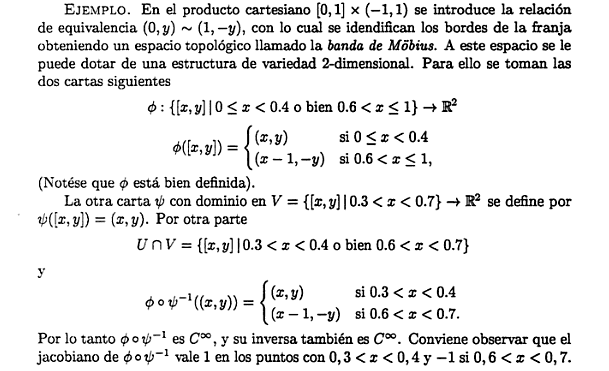
\includegraphics[keepaspectratio=true,width=\linewidth]{img/ejemplo_6.png}
\end{center}

Para dotar a un conjunto de estructura diferencial basta con encontrar un atlas para el cual se cumpla la definición de estructura diferencial sobre el conjunto dado.

Tomamos 8 cartas de la siguiente forma:
\begin{enumerate}
\item
\[\appl{\phi_1}{\{(x,y,z) \tq x\in [0,1), y \in [0,1), z \geq 0\}}{\real^3}\]
siendo $\phi_1=Id$
\item
\[\appl{\phi_2}{\{(x,y,z) \tq x\in (-1,0], y \in [0,1), z \geq 0\}}{\real^3}\]
siendo $\phi_2((x,y,z)=(-x,y,z)$
\item
\[\appl{\phi_3}{\{(x,y,z) \tq x\in [0,1), y \in (-1,0], z \geq 0\}}{\real^3}\]
siendo $\phi_3((x,y,z)=(x,-y,z)$
\item
\[\appl{\phi_4}{\{(x,y,z) \tq x\in [0,1), y \in [0,1), z < 0\}}{\real^3}\]
siendo $\phi_4((x,y,z)=(x,y,-z)$
\item
\[\appl{\phi_5}{\{(x,y,z) \tq x\in (-1,0], y \in (-1,0], z \geq 0\}}{\real^3}\]
siendo $\phi_5((x,y,z)=(-x,-y,z)$
\item
\[\appl{\phi_6}{\{(x,y,z) \tq x\in (-1,0], y \in [0,1), z < 0\}}{\real^3}\]
siendo $\phi_6((x,y,z)=(-x,y,-z)$
\item
\[\appl{\phi_7}{\{(x,y,z) \tq x\in [0,1), y \in (-1,0], z < 0\}}{\real^3}\]
siendo $\phi_7((x,y,z)=(x,-y,-z)$
\item
\[\appl{\phi_8}{\{(x,y,z) \tq x\in (-1,0], y \in (-1,0], z < 0\}}{\real^3}\]
siendo $\phi_8((x,y,z)=(-x,-y,-z)$

\end{enumerate}

La combinación de una de estas funciones con la inversa de otra no implicará más que cambios de signo sobre las variables de tal forma que
\[\phi_i\circ \inv{\phi_j}(x,y,z)=(\pm x, \pm y, \pm z\]
y queda claro que estas aplicaciones son $C^{\infty}$ y sus inversas, que son de la misma forma, también. Conviene observar que el jacobiano vale siempre $\pm 1$
\end{problem}

\section{fasc-4-ejemplos}

\subsection{Variedades}
\begin{problem}[2]
Estudiar, siguiendo el modelo de $S^2$ la estructura de variedad diferenciable, con dos cartas, en $S^n$

\solution
\textcolor{blue}{Hecho por Pedro. No fiarse al 100\%}

Comenzamos considerando una esfera de radio 1 en $\real^n$ que tendrá la ecuación:
\[\sum_{i=1}^n x_i^2=1\]
y describiendo explícitamente el atlas de dos cartas dado por la proyección estereográfica.

Siguiendo el ejemplo de la hoja, consideramos la proyección tomando el polo norte $(1,0...0)$ y el plano $x_1=-1$. Posteriormente construiremos la segunda carta tomando el polo sur $(-1,0...0)$ y el plano $x_1=1$. Vamos a ello.

\textbf{Primera carta}

\begin{itemize}
\item Supongamos un punto $p$ cualquiera del plano $x_1=-1$:
\[p=(-1,x_2,...x_n)\]

Si construimos la recta que lo une con el polo norte y la intersecamos con la esfera $S^n$ obtenemos el punto intersección $q$.
\[q = \left(1-2t, x_2\cdot t,...,x_n\cdot t\right)\]
Si el punto es la intersección con la esfera, su módulo deberá ser 1. Utilizamos este dato para calcular $t$.

\[1+4t^2-4t+t^2\left(\sum_{i=2}^nx_i^2\right)=1 \implies 4t^2-4t+t^2\left(\sum_{i=2}^nx_i^2\right) = 0 \implies t=\frac{4}{\sum_{i=2}^nx_i^2+4}\]

Por tanto el punto de intersección es:
\[q=\left(1-\frac{8}{\sum_{i=2}^nx_i^2+4}, \frac{4x_2}{\sum_{i=2}^nx_i^2+4},...,\frac{4x_n}{\sum_{i=2}^nx_i^2+4} \right)\]

\item Al revés. Empezamos ahora con un punto
\[x\in S^n\tq x=(α_1...α_n) \text{ con } \sum_{i=1}^n α_i^2 = 1\]

Construimos ahora el vector que une este punto con el polo norte y lo intersecamos con el plano $x_1=-1$

La recta unión con el polo norte queda de la forma:
\[\left(1+t(α_1+1),α_2t,...,α_nt \right)\]
y forzamos la intersección de esta recta con el plano para conocer el punto
\[1+t(α_1+1)=-1 \implies t = \frac{-2}{α_1+1}\]
con lo que el punto sería:
\[\left( -1, \frac{-2α_2}{α_1-1}, ..., \frac{-2α_n}{α_1-1}\right)=\left( -1, \frac{2α_2}{1-α_1}, ..., \frac{2α_n}{1-α_1}\right)\footnote{En el ejmplo de la hoja creo que escriben $α_1$ en función de las otras coordenadas, pero no veo necesaria esta complicación}\]
\end{itemize}

\textbf{Segunda carta}
\begin{itemize}
\item Supongamos un punto $p$ cualquiera del plano $x_1=1$:
\[p=(1,x_2,...x_n)\]

Si construimos la recta que lo une con el polo sur y la intersecamos con la esfera $S^n$ obtenemos el punto intersección $q$.
\[q = \left(-1+2t, x_2\cdot t,...,x_n\cdot t\right)\]
Si el punto es la intersección con la esfera, su módulo deberá ser 1. Utilizamos este dato para calcular $t$.

\[1+4t^2-4t+t^2\left(\sum_{i=2}^nx_i^2\right)=1 \implies 4t^2-4t+t^2\left(\sum_{i=2}^nx_i^2\right) = 0 \implies t=\frac{4}{\sum_{i=2}^nx_i^2+4}\]

Por tanto el punto de intersección es:
\[q=\left(-1+\frac{8}{\sum_{i=2}^nx_i^2+4}, \frac{4x_2}{\sum_{i=2}^nx_i^2+4},...,\frac{4x_n}{\sum_{i=2}^nx_i^2+4} \right)\]

\item Al revés. Empezamos ahora con un punto
\[x\in S^n\tq x=(α_1...α_n) \text{ con } \sum_{i=1}^n α_i^2 = 1\]

Construimos ahora el vector que une este punto con el polo sur y lo intersecamos con el plano $x_1=1$

La recta unión con el polo sur queda de la forma:
\[\left(-1+t(α_1+1),α_2t,...,α_nt \right)\]
y forzamos la intersección de esta recta con el plano para conocer el punto
\[-1+t(α_1+1)=1 \implies t = \frac{2}{α_1+1}\]
con lo que el punto sería:
\[\left( 1, \frac{-2α_2}{α_1+1}, ..., \frac{-2α_n}{α_1+1}\right))\]
\end{itemize}

Estudiamos ahora un punto cualquiera del plano $(-1,...x_n)$. Si lo mandamos en la esfera por la primera proyección que hemos calculado, llegamos al punto
\[\left(1-\frac{8}{\sum_{i=2}^nx_i^2+4}, \frac{4x_2}{\sum_{i=2}^nx_i^2+4},...,\frac{4x_n}{\sum_{i=2}^nx_i^2+4} \right)\]

Ahora calculamos la imagen directa de este punto por la segunda proyección estereográfica, con lo que llegamos a:
\[\left( 1, \frac{-2\frac{4x_2}{\sum_{i=2}^nx_i^2+4}}{2-\frac{8}{\sum_{i=2}^nx_i^2+4}}, ..., \frac{-2\frac{4x_n}{\sum_{i=2}^nx_i^2+4}}{2-\frac{8}{\sum_{i=2}^nx_i^2+4}}\right)=\left( 1, \frac{-4x_2}{\sum_{i=2}^nx_i^2},...,\frac{-4x_n}{\sum_{i=2}^nx_i^2}\right)\]

y podemos ver que se trata de un difeomorfismo sobre su imagen

\textcolor{blue}{En algún punto he metido la gamba con los signos porque debería salirme todo positivo. Pero ya he currado mucho con este ejercicio. Una paja y a seguir.}

\end{problem}



\begin{problem}[3]
Parametrizamos los puntos del hemisferio norte de la esfera $x_2 > 0$,
excluyendo el ecuador ($x_2 = 0$), en la forma $(θ, τ, + \sqrt{1 − θ^2 − τ^2})$ con
$θ^2 + τ^2 < 1$. Esto convierte al hemisferio norte en una carta coordenada, y podemos cubrir la esfera con seis cartas de este tipo tomando
como ecuador cada una de las intersecciones de la esfera con los planos
coordenados. COMPROBAR que, efectivamente, se trata de un atlas.

DEMOSTRAR que los dos atlas son equivalentes, viendo que los cambios
de carta de una carta de uno de ellos a una carta del otro inducen difeomorfismos.

\solution
\end{problem}

\begin{problem}[4]
Demostrar que no existe ninguna variedad diferenciable compacta que se pueda recubrir con una única carta coordenada
\solution

\textcolor{blue}{Hecho por mi. No fiarse al 100\%}

Si una variedad se puede recubrir por una única carta será homeomorfa a un abierto de $\real^n$ y, consecuentemente, nunca podrá ser compacta.

Esta respuestá está basada en la proposición 1.28 del documento: \href{http://ocw.um.es/ciencias/geometria-y-topologia/material-de-clase-1/01-variedadesdiferenciablessubvariedades-v100901.pdf}{Variedades Diferenciales y Subvariedades.pdf}
\end{problem}

\begin{problem}[5]
Demostrar que toda variedad 1-dimensional compacta y conexa es difeomorfa a la circunferencia $S^2$
\solution

\textcolor{blue}{Hecho por mi. No fiarse al 100\%}

Para empezar es obvio que en caso de haber un difeomorfismo entre una variedad y la circunferencia, la variedad ha de ser compacta y conexa, pues así lo es la circunferencia.

Para resolver este ejercicio me baso en la proposición \href{https://books.google.es/books?id=CAOjRFAMJFUC&pg=PA131&lpg=PA131&dq=variedad+1-dimensional&source=bl&ots=MLkMP7HMyo&sig=aLLSSaYknqPZhPsn-5jJM2MwPAc&hl=es&sa=X&ei=DeMeVZSOEczZPdLkgfgJ&ved=0CCcQ6AEwAQ#v=onepage&q&f=false}{VI.1.6}. Básicamente la copio como un bellaco pero ahí dejo el link para el que quiera profundizar.

\textcolor{blue}{Justo en la versión que se puede consultar gratis en Google han quitado las dos páginas clave en que salía esto. El lunes pillo el libro en ciencias y lo completo}

\end{problem}

\begin{problem}[6]
Demostrar, como consecuencia del teorema de invarianza del dominio, que si $n \neq m$, no pueden ser homeomorfos $\real^n$ y $\real^m$. Tampoco es posible que sean homeomorfos un abierto de $\real^n$ con uno de $\real^m$
\solution

\textcolor{blue}{Hecho por Pedro. No fiarse al 100\%}

La solución se ha obtenido de este \href{http://www.cmat.edu.uy/~rpotrie/documentos/pdfs/invarianciadimension.pdf}{documentopdf}

\textcolor{blue}{Esta demostración se hace prácticamente usando los conocimiento del curso de Topología y no veo una forma clara de hacerlo con lo estudiado en este curso de Geometría Diferencial.}
\end{problem}

\begin{problem}[7]
Demostrar que, si $\appl{f}{M}{N}$ es una función continua y localmente inyectiva de variedades topologícas de dimensión $n$, entonces la imagen de todo abierto $U \subset M$ es un abierto de $N$. En particular, $f(M)\subset N$ debe ser un abierto, que puede ser toda la variedad $N$
\solution

\textcolor{blue}{Hecho por Pedro. No fiarse al 100\%}

Esto es un resultado de Topología que no voy a rehacer ya que no le veo mucha relación con lo que estamos estudiando en esta asignatura.

Por comentar algo relacionado con lo que estamos viendo, he viso en Wikipedia, y cito textualmente: ``El teorema de la invariancia del dominio establece que una función continua y localmente inyectiva entre dos variedades topológicas n-dimensionales debe ser abierta.''
\end{problem}

\begin{problem}[8]
Sea $S$ el conjunto de sucesiones $\appl{σ}{\nat}{\real}$ de números reales.

Definimos una topología en $S$ exigiendo que todas las funciones naturales de proyección
\[\appl{μ_{i_1,i_2,...,i_n}}{S}{\real^n}\]
sean continuas.\footnote{Estas funciones básicamente llevan la sucesión a un vector de $\real^n$ formado por $n$ elementos de la sucesión.}

Definimos una función $\appl{F}{S}{S}$ mediante
\[F(x_0,x_1,...,x_n,...)=(x_1,x_2,...,x_n,...)\]
Demostrar que la función $F$ es continua e inyectia, pero su imagen no es un abierto de $S$

\solution


\end{problem}

\begin{problem}[9]
Sea $U$ una bola unidad abierta en $\real^n$. Comprobar que la aplicación
\[f(\vx)=\frac{\vx}{\sqrt{1-\norm{\vx}^2}}\]
es un difeomorfismo de $U$ en todo $\real^n$
\solution

\yoP

Para comprobar que $f$ es un difeomorfismo debemos ver que es diferenciable, biyectiva y con inversa diferenciable. Vamos a ello.

La función, descompuesta en coordenadas, queda de la forma:
\[f(\vx)=\left(\frac{x_1}{\sqrt{1-\norm{\vx}}}, \frac{x_2}{\sqrt{1-\norm{\vx}}}, ..., \frac{x_n}{\sqrt{1-\norm{\vx}}}\right)\]

Vamos a derivarla:
\[\frac{\partial f}{\partial x_i}=\left(\frac{x_1x_i}{(\sqrt{1-\norm{\vx}})^3},\frac{x_2x_i}{(\sqrt{1-\norm{\vx}})^3},..\frac{1}{\sqrt{1-\norm{\vx}}}+\frac{x_i^2}{(\sqrt{1-\norm{\vx}})^3}.,\frac{x_nx_i}{(\sqrt{1-\norm{\vx}})^3}\right)\]

Podemos observar que la derivada existe (y por tanto la función es diferenciable) en todo punto con norma distinta de 1. Puesto que nos estamos restringiendo a $U$ que es la bola unidad \textbf{abierta} no hay problema con esto.

Podemos ver de manera sencilla que la función es inyectvia pues la derivada nunca se anula y podemos ver que es sobreyectiva por contrucción. Para cualquier punto de $\real^n$ que tomemos podemos escribirlo como $f(\vx)$\footnote{Esto queda claro al calcular la función inversa, cosa que haremos a continuación}.

Por último nos queda estudiar la inversa.

\[f(\vx)=\vy \implies (y_1,....y_n)=\left(\frac{x_1}{\sqrt{1-\norm{\vx}}}, \frac{x_2}{\sqrt{1-\norm{\vx}}}, ..., \frac{x_n}{\sqrt{1-\norm{\vx}}}\right)\]

A ojo de buen cubero podemos ver que la función inversa sería
\[f^{-1}(\vy)=\frac{\vy}{\sqrt{1+\norm{\vy}}}\]
cosa que podemos comprobar fácilmente.

Resulta también trivial la observación de que esta función inversa también es diferenciable, por lo que queda claro que $f$ es un difeomorfismo.

\end{problem}


\subsection{Campos}
\begin{problem}[1]
(\textbf{Grupos uniparamétricos de automorfismos}) En cada uno de los siguientes ejemplos se da una familia uniparamétrica de automorfismos de $\real^n$ y se pide que se compruebe que es un grupo y determine el campo asociado (\textbf{generador infinitesimal del grupo}). En todos los casos el grupo es un grupo de transformaciones lineales y el campo es un campo lineal (coeficientes de grado a lo más uno)

\ppart Grupo de traslaciones
\[τ_1(x_1,...,x_n)=(x_1+t,x_2,...,x_n)\]

\ppart Grupo de homotecias
\[τ_t(x_1,...,x_n)=(e^tx_1, e^tx_2,...,e^tx_n\]

\ppart Sea $A$ una matriz $n\times n$. Definimo un grupo uniparamétrico de automorfismos, asociado a la matriz $A$, mediante
\[τ_t(X)=e^{tA}X\]
¿Es el primer ejemplo un caso particular de este?

\ppart
Supongamos ahora $n=2$, y sea
\[ \left( \begin{array}{cc}

\cos(t) & -\sin(t) \\
\sin(t) & \cos(t)

\end{array} \right)\]
la matriz de una rotación de ángulo variable $t$ en el plano. Definimos un grupo uniparamétrico de automorfismos
\[τ_t(x_1,x_2)=A(t)\cdot {x_1 \choose x_2}\]

¿Es este ejemplo un caso particular del c)?

\solution
\yoP

Para demostrar que cada uno de estos conjuntos es un grupo debemos identificar la operación que define el grupo, demostrar que es asociativa y encontrar el elemento neutro o identidad y el inverso.

\spart
La operación suma se define de la siguiente forma:
\[(τ_a+τ_b)(x_1,...,x_n)=(x_1+a+b,x_2,...,x_n)\]

Es evidente que la operación es asociativa, el elemento neutro es $τ_0$ y el inverso de $τ_t$ es $τ_{-t}$

Queda claro que es un grupo.

Vamos a encontrar el campo asociado. La teoría de lo que vamos a hacer a continuación viene en las páginas 73-74 de \href{http://matematicas.unex.es/~ricarfr/EcDiferenciales/LibroEDLat.pdf}{documento.pdf}

Básicamente nos da un teorema y su demostración. El teorema dice:

Sea $X$ un grupo uniparamétrico local de clase $k$. Para cada $f\in C^{\infty}(U)$ y $p \in U$ definimos
\[(Df)(p)=\lim_{t \to 0}\frac{f[X(t,p)]-f(p)}{t}\]
entonces $D \in D_k(U)$ y lo llamaremos generador infinitesimal de X.

El ejemplo concreto que vamos a hacer (o uno muy similar) así como los siguientes vienen resuletos al final de la página 16 de \href{http://matematicas.unex.es/~ricarfr/EcDiferenciales/LibroEDLat.pdf}{documento.pdf}

Así para este ejemplo tendríamos la aplicación flujo $\appl{\phi}{\real^{n+1}}{\real^n}$ siendo $\phi(x_1,...,x_n,t)=(x_1+t,x_2,...,x_n)$.

\[X = \left(\frac{\partial \phi}{\partial t}\right)_{t=0} \frac{\partial}{\partial x_i}=\frac{\partial}{\partial x}\]


\textbf{Del último documento mencionado cabe destacar:}

\begin{defn}[Generador infinitesimal]
Sea $\{σ_t\}$ un grupo monoparamétrico de transformaciones de U. Llamamos \textbf{generador infinitesimal} de $\{σ_t\}$ al campo vectorial que asigna al punto $p$, el vector tangente a la curva $(-ε,ε)\to U$, $t \to σ_t(p)$

Consideremos $\appl{\phi}{\real \times U}{U}$ la aplicación flujo del grupo $\phi(t,p)=σ_t(p)$. entonces el generador infinitesimal puede considerarse
\[X = \sum_{i=1}^n \left( \frac{\partial \phi_i}{\partial t}\right)_{t=0}\frac{\partial}{\partial x_i}\]
\end{defn}

\end{problem}

\begin{problem}[2]
Sea $D$ el campo en $\real^2$ definido como
\[D=x \frac{\partial}{\partial x}+y \frac{\partial}{\partial y }\]

El campo está definido en tdo el plano pero

\ppart Una integral primera definida en todo el plano es necesariamente constante

\ppart Para cada punto, diferente al origen hay un entorno en el que hay una integral primera. Determnar todas esas integrales primeras no globales y los abiertos máximos en que están definidas.
\solution
\end{problem}

\begin{problem}[3]
Estudiar el campo en el plano definido como
\[D=(y+x(1-x^2-y^2))\frac{\partial}{\partial x} + (-x+y(1-x^2-y^2))\frac{\partial}{\partial y}\]
usando, si te parece conveniente, un cambio a coordenadas polares.
\solution

\end{problem}


\chapter{Discusiones interesantes}

\section{Funciones suaves no analíticas}

\begin{figure}[hbtp]
\centering
\inputtikz{Ap_SuaveNoAnalitica}
\caption{Una función suave no analítica, dada por $f(x) = 0$ cuando $x ≤ 0$ y $f(x) = e^{\frac{-1}{x}}$ cuando $x > 0$. $f$ se anula en el origen y todas sus derivadas también, pero $f$ no es nula.}
\end{figure}

En la sección \ref{secDimTangente} hablábamos de anillos, y surge la pregunta de si esos anillos de funciones son también dominios. No lo son por la existencia de divisores de cero: funciones suaves no analíticas.

Estas funciones son $C^∞$ con $f^{(n)}(x) = 0\; ∀n$, pero $f ≠ 0$, una contradicción aparente ya que su desarrollo de Taylor con todas las derivadas nulas sería idénticamente nulo.

En Wikipedia \href{http://en.wikipedia.org/wiki/Non-analytic_smooth_function}{hay una discusión más detallada sobre este tema}.

\chapter{Definiciones adicionales}

\begin{defn}[Delta\IS de Kronecker] \label{defDeltaKronecker} La delta de Kronecker se define como \[ δ_{ij} = \begin{cases} 0 & i ≠ j \\ 1 & i = j \end{cases} \] \end{defn}

\begin{theorem} [Teorema\IS de la función inversa] \label{thmInv} Sea $\appl{F}{\Omega\subset\real^N}{\real^N} \text{ con } F\in C^1(\Omega)$.

Supongamos $DF(\ga)$ invertible, $\ga \in \Omega$. Entonces existe un abierto $V \tlq F(\ga)\in V$, un abierto $U \tlq \ga \in U$ y una inversa local $\appl{G}{V}{U}$. Además, $G$ es diferenciable en $U$ y

\[ DG(y) = \left[DF(\F(y))\right]^{-1}, \forall y \in U \]
\end{theorem}

\begin{theorem}[Teorema\IS de la función implícita] \label{thmFImp} Dadas $n$ ecuaciones, $n+m$ incógnitas, consideramos

$$\appl{F}{\Omega\subset\underbrace{\real^M}_{x,y} \times \underbrace{\real^N}_{z}}{\real^N}$$

Supongamos $F\in C^1$. Sea $\ga \in \real^M, \gor{b} \in \real^N \tlq (\gor{a},\gor{b})\in \Omega , F(a,b)=0$. Supongamos $D_yF(\ga,\gb)$ no singular, $\det(D_yF)\neq 0$. Entonces existen abiertos $\omega \subset \real^M, \Theta \in\real^n$, con $\ga \in \omega, \gb \in \Theta$ y una única función: \[ \appl{g}{\omega\subset\real^M}{\Theta \subset\real^N}, g\in C^1(\omega) \]

que cumple

\[ g(\ga) = \gb;\; F(\gx,g(\gx)) = \gor{0}\; \forall \gx \in \omega \]
\[ Dg(\gx) = - \left[D_yF(\gx,g(\gx))\right]^{-1} \cdot D_xF(\gx,g(\gx)) \]
\end{theorem}

\begin{defn}[Difeomorfismo] Se dice que $\appl{F}{A}{B}$ es difeomorfismo si es biyectiva, derivable y con inversa derivable. \label{defDifeomorfismo}
\end{defn}

\printindex
\end{document}
